\documentclass[chi_draft]{sigchi}

% Use this command to override the default ACM copyright statement
% (e.g. for preprints).  Consult the conference website for the
% camera-ready copyright statement.

%% EXAMPLE BEGIN -- HOW TO OVERRIDE THE DEFAULT COPYRIGHT STRIP -- (July 22, 2013 - Paul Baumann)
% \toappear{Permission to make digital or hard copies of all or part of this work for personal or classroom use is      granted without fee provided that copies are not made or distributed for profit or commercial advantage and that copies bear this notice and the full citation on the first page. Copyrights for components of this work owned by others than ACM must be honored. Abstracting with credit is permitted. To copy otherwise, or republish, to post on servers or to redistribute to lists, requires prior specific permission and/or a fee. Request permissions from permissions@acm.org. \\
% {\emph{CHI'14}}, April 26--May 1, 2014, Toronto, Canada. \\
% Copyright \copyright~2014 ACM ISBN/14/04...\$15.00. \\
% DOI string from ACM form confirmation}
%% EXAMPLE END -- HOW TO OVERRIDE THE DEFAULT COPYRIGHT STRIP -- (July 22, 2013 - Paul Baumann)

% Arabic page numbers for submission.  Remove this line to eliminate
% page numbers for the camera ready copy
\pagenumbering{arabic}

% Load basic packages
\usepackage{balance}  % to better equalize the last page
%\usepackage{graphics} % for EPS, load graphicx instead 
\usepackage{graphicx}
\usepackage[labelfont={bf},textfont={bf},font=small]{caption}
\usepackage[labelfont={bf},textfont={bf},font=small]{subcaption} % if two images are rigth next to eachother
\usepackage[T1]{fontenc}
\usepackage{txfonts}
\usepackage{mathptmx}
\usepackage[pdftex]{hyperref}
\usepackage{color}
\usepackage{booktabs}
\usepackage{textcomp}
% Some optional stuff you might like/need.
\usepackage{microtype} % Improved Tracking and Kerning
% \usepackage[all]{hypcap}  % Fixes bug in hyperref caption linking
\usepackage{ccicons}  % Cite your images correctly!
\usepackage[utf8]{inputenc} % for a UTF8 editor only
\usepackage{tikz}
\newcommand*\circled[1]{\tikz[baseline=(char.base)]{
            \node[shape=circle,draw,inner sep=2pt] (char) {#1};}} % circled icons for image citation
						
% If you want to use todo notes, marginpars etc. during creation of your draft document, you
% have to enable the "chi_draft" option for the document class. To do this, change the very first
% line to: "\documentclass[chi_draft]{sigchi}". You can then place todo notes by using the "\todo{...}"
% command. Make sure to disable the draft option again before submitting your final document.
\usepackage[backgroundcolor=yellow,textsize=small]{todonotes}
\usepackage{blindtext}

% Paper metadata (use plain text, for PDF inclusion and later
% re-using, if desired).  Use \emtpyauthor when submitting for review
% so you remain anonymous.
\def\authorname{Tobias Lahmann}
\def\plaintitle{Games in VR}
\def\plainauthor{\authorname}
\def\emptyauthor{}
\def\plainkeywords{Virtual reality, games, psychology, research}
\def\plaingeneralterms{Documentation, Standardization}

% llt: Define a global style for URLs, rather that the default one
\makeatletter
\def\url@leostyle{%
  \@ifundefined{selectfont}{
    \def\UrlFont{\sf}
  }{
    \def\UrlFont{\small\bf\ttfamily}
  }}
\makeatother
\urlstyle{leo}

% To make various LaTeX processors do the right thing with page size.
\def\pprw{8.5in}
\def\pprh{11in}
\special{papersize=\pprw,\pprh}
\setlength{\paperwidth}{\pprw}
\setlength{\paperheight}{\pprh}
\setlength{\pdfpagewidth}{\pprw}
\setlength{\pdfpageheight}{\pprh}

% Make sure hyperref comes last of your loaded packages, to give it a
% fighting chance of not being over-written, since its job is to
% redefine many LaTeX commands.
\definecolor{linkColor}{RGB}{6,125,233}
\hypersetup{%
  pdftitle={\plaintitle},
  pdfauthor={\plainauthor},
%  pdfauthor={\emptyauthor},
  pdfkeywords={\plainkeywords},
  bookmarksnumbered,
  pdfstartview={FitH},
  colorlinks,
  citecolor=black,
  filecolor=black,
  linkcolor=black,
  urlcolor=linkColor,
  breaklinks=true,
}

% create a shortcut to typeset table headings
% \newcommand\tabhead[1]{\small\textbf{#1}}

% End of preamble. Here it comes the document.
\begin{document}

\title{\plaintitle}

\numberofauthors{1}
\author{
	\alignauthor{\authorname\\
		\affaddr{Ulm University}\\
		\affaddr{Ulm, Germany}\\
		\email{tobias.lahmann@uni-ulm.de}}
%	\alignauthor{Julian Frommel\\
%		\affaddr{Research Trends in Media Informatics}\\
%		\affaddr{Ulm, Germany}\\
%		\email{julian.frommel@uni-ulm.de}}
}

\maketitle
\todo[inline]{need a better title}

%----------------------------------------------------------------------------------------
%	Document
%----------------------------------------------------------------------------------------
Lieber Interessierter,

ich habe leider keine Ahnung wie das Proposal im endeffekt aussehen soll. Hier mal die Struktur, die Inhalte und die Referenzen, die ich mir so vorstelle.

Ich wünsche viel Spaß beim Lesen

-TL

\begin{abstract}
Virtual Reality techniques are very well suited for games as they incorporate users into the action and offer great potential for developers to extend the experience conveyed in their games. Understanding the advantages but also the disadvantages of VR in all fields of gaming is important for the future advancement of the fields.
The many varying aspects and different field of needed research for \textit{Games in VR} will be examined here.
Other literature is often focusing either on the field of games and analyzing the game-impacts on players or the psychological affects of games, or is studying the field of virtual reality and the affects of this.
The objective of this publication is to combine both fields and show future development of games in virtual reality.
\end{abstract}


\category{H.5.1}{[Multimedia Information Systems]: Artificial, augmented, and virtual realities}{}{}

\keywords{\plainkeywords}


\section{Introduction}
%\todo[inline]{write introduction}

The virtual generation and perception of real environments or imaginary settings, rendered by a computer using specialized software, is referred to as virtual reality (VR). Its goal is to simulate a user's physical presence in this environment, by enabling the user to interact with this space and any objects depicted therein using specialized display screens or projectors and other devices.

The potential of virtual reality in gaming is an enormous factor both for the scientific and commercial regarding its multitude of use cases. 

In the past decade a variety of electronic devices has reached the marked and found its way into the homes of consumers. Gaming consoles have become entertainment systems offering more than just the gaming aspect. Computers gained the abilities of past supercomputers and are far more than workstations for the majority of modern population. With technological advancements made in the past 50 Years and popularity gains of these systems also the gaming industry has reached its heyday. 

VR, although expensive, gains more interest and the audience grows almost daily. 
Games that do not naturally support VR are searching for ways to include VR in their games, described in the section \textit{Games And VR}\ref{sec:gamesNvr}.

\begin{figure}%[h]
	\centering
	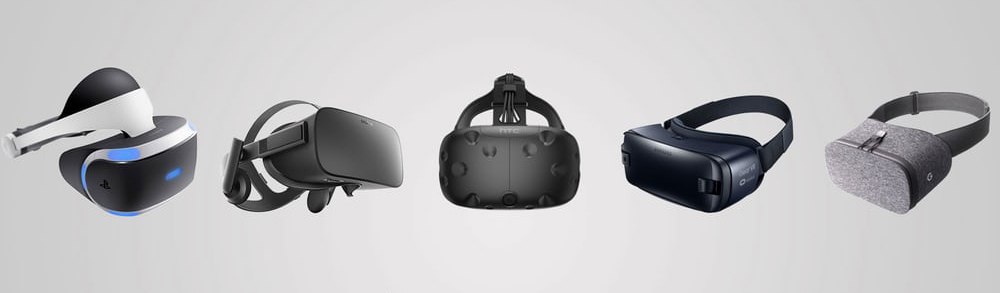
\includegraphics[width=0.99\columnwidth]{./figures/vr-hmd}
	\caption[vr-hmd]{Overview of different consumer HMD as available in late 2016. FLTR Plystation VR, Oculus Rift, HTC Vive, Samsung Gear VR, Daydream View.\footnotemark}~\label{fig:vrHMD}
\end{figure}
\footnotetext{\textcopyright~Newatlas, [Online; accessed January 04., 2017],[Digitally revised] \url{http://img-2.newatlas.com/vr-comparison-2016-b-2.jpg}}

The development of consumer friendly head mounted devices (HMD) for VR, as to see in \textbf{Figure~\ref{fig:vrHMD}}, has just picked up in recent years with systems like the \textit{Oculus Rift in March 2016}, the \textit{HTC Vive in April 2016}, the \textit{Samsung Gear VR in August 2015}, the \textit{Playstation VR in October 2015} or the \textit{Daydream View in November 2015}. 

Many developers have already started to develop games that use the advances of VR and are serving quick, but the research on this fields has lacked behind on reliable results regarding the ideal approach to points such as immersion, interaction and performance. This publication intends to show the many disciplines and what research can be done to improve VR in Games.



\todo[inline]{existing game research?? own section?}

\section{Games and the Virtual Reality}

\todo[inline]{JF: Die Wahl wirkt trotzdem ein bisschen willkürlich

Außerdem gibts The Lab nur für die Vive und nicht "regulär", Dota2 für VR ist auch nicht wirklich vergleichbar da das nur der Spectator Mode ist, Minecraft passt ganz gut als Vergleich aber da ist es auch noch unterschiedlich: Für die Vive gibt es nur Hacks, aber die Steuerung wird natürlich gut ausgenutzt. Gear und Oculus werden offiziell unterstützt aber da funktioniert die Interaktion anders als bei der Vive.

Zu FM 2017 hab ich jetzt nur Ankündigungen gefunden. Gibt's denn da was in VR?}
\begin{table}[h]
	\caption{Popular games played in late 2016. The games offer a regular play mode, using the monitor, and a VR play mode. Games are chosen from different genres to compare the influence from and to virtual reality.}~\label{tab:popularGames}
	
	%{}\fontfamily{pcr}\selectfont
	\begin{tabular*}{\columnwidth}{ l l r r }
		Gametitle & Genre\footnotemark & \parbox[c][2.2em][t]{2cm}{\begin{flushright}$\dfrac{Players}{Month}$(\footnotemark)\end{flushright}} & Metascore\footnotemark \\
		\hline
		The Lab & Puzzle & 0.16 K & 74 \\
		Dota 2 & MOBA & 611 K & 90 \\
		%Counter Strike: GO & FPS & 330 & 83 \\
		Minecraft & RPG & 300 K & 93 \\
		Superhot (VR) & FPS & 0.19 K & 83 \\
		Football Mgr. '17 & Sports & 15 K & 79 \\
	\end{tabular*}
	%}
	
\end{table}

\todo[inline]{table too small?}
\footnotetext{MOBA: Multiplayer Online Battle Arena; FPS: First-Person Shooter; RPG: Role-Playing Game}
\footnotetext{\url{http://steamcharts.com}, accessed Nov. 12., 2016}
\footnotetext{\url{http://www.metacritic.com}, accessed Nov. 12., 2016}
\todo[inline]{Die footnotes werden nicht richtig nummeriert... von hand fixen bei submission!?}


Write something about the motivation in games of Table~\ref{tab:popularGames}. Why are the games good or bad to play with VR and why the games are popular. Write about the movement of the player in the games. Write about the physics, the game principles and the differences to solely non-vr games.

\subsection{Popularity Of Games}
Since the beginning of virtual reality in late \textcolor{red}{20th century} there has been a huge potential to include the user in a virtual environment. Some systems have been developed in the past century that simplify some processes of work for different disciplines. 

Games have just lately adopted the potential for this immersive form of gaming and with the developement of the \textcolor{red}{\textit{Oculus Rift in 2014}}, the \textcolor{red}{\textit{HTC Vive in 2016}}, and the \textcolor{red}{\textit{Samsung Gear in 2015}} and the \textcolor{red}{damit einhergehend} distribution of these systems into the living room of many people.

In \textcolor{red}{gegensatz/ parallel dazu} the research on these fields has not made huge advances with the field.

PAPER on gaming addictions and popularity of games

Games using a virtual environment to show worlds to players give the player the feeling of being in the middle of the happening(?) but the game has very limited possibilities to tell storys with much varity, because the game can not change perspectives as easy. \textcolor{red}{\textit{wohingegen} games that do not use VR can handle attention themself by just moving the camera. these games can show views from other perspective without worriing about the user being confused too much. VR-Games need another way to handle interaction, i.e. the user has to hold some kind of controller interface to tell the system what he wants to do. Games outside of vr have similar interface problems but the process has been researched more than the interaction with VR-Games. \textcolor{red}{\textit{gleichzeitig} do vr-games \textcolor{red}{\textit{fordern} a much more active way of interaction, because the user has to complete different tasks as he is playing the game. this can be a negative point for people who would just rather enjoy a game than have a minor workout while playing.
			
pro vr: immerse, active, intuitive, innovative.
contra vr: active, expensive, hard to develop games

Why VR games are as popular as they are

\todo[inline]{JF: Auch oder vielleicht sogar mehr: Wieso nicht? Ist es nur dass die Technologie noch nicht verbreitet genug ist? Machen die Spiele was anders? Funktionieren traditionelle Spiele nicht einfach so in VR? etc.}

\subsection{Motivation In Games}
What Motivation can VR offer that other Games cannot offer. What motivation can normal games offer, that vr-games cannot offer.

motivation of players: (talk)\footnote{"Gamer Motivation Profile Findings - \#GamesUR US Conference 2016" Quantic Foundry Website, March, 25., 2015, accessed November 05., 2016, \url{http://quanticfoundry.com/2016/04/07/gdc-talk/}}
\begin{itemize}
	\item action
	\item social
	\item mastery
	\item achievement
	\item immersion
	\item creativity
	\item \textbf{age}
\end{itemize}

\subsection{Games Exclusively For VR}
Why games are developed solely for VR


\section{Input Techniques}

Oculus Rift

HTC Vive

Samsung Gear

Dancing in front of a camera. XBox camera stuff

what research has been done. how can input be changes. what adjustments are possible. what adjustments are necessary. How can a user be teached what to do if some things happen. what generic input of interaction methods can be defined beween systems.

what other channel of interaction can be used (sound, video)


\section{Further research trends}
\subsection{Physical And Mental Aspects}

Ranasinghe, Nimesha and Do, Ellen Yi-Luen have developed a way to address the tastebuds using electrical stimulation \cite{Ranasinghe:2016:VSS:2984751.2985729}

Health care training for professional workers in health-care

People could be treated with games, regarding the profits of arcieving womething, and VR, the profit of feeling right in the middle of the happening

cyber sickness is a large field, witch should be researched because, weh the people dont move but the eyes tell the brain that they are moving, it becomes confused (similar to sea-sickness)

motivation of players: (talk)\footnote{"Gamer Motivation Profile Findings - \#GamesUR US Conference 2016" Quantic Foundry Website, March, 25., 2015, accessed November 05., 2016, \url{http://quanticfoundry.com/2016/04/07/gdc-talk/}}
\begin{itemize}
	\item action
	\item social
	\item mastery
	\item achievement
	\item immersion
	\item creativity
\end{itemize}

%\textcolor{gray}{\blindtext[3]}

\subsection{Physical Objects}

Using some similar technology to the iDummy\footnote{"IDummy" IDummy Product Website, 2015, accessed November 05., 2016, \url{http://www.idummy.com/}} one can create various objects of different size and shape. A user wearing a VR Headset can see a specific object and feel it as if it was the real thing. Using the technology developers can extend the realm of VR to one more dimension. Together with the technology~\cite{Azmandian:2016:HRD:2858036.2858226}

Using something similar to the modular tiles creating levels in portal (a 100x100 cm tile is attached to a robotic arm)

\begin{figure}
	\centering
	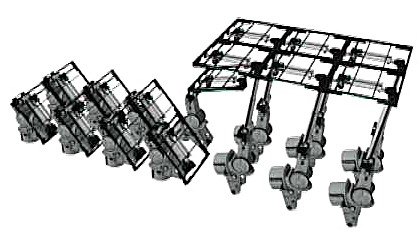
\includegraphics[width=0.9\columnwidth]{./figures/portallabrattest}
	\caption[Portal 2 : Lab Rat Panel Test]{Screenshot from the promotional video 'Portal 2 : Lab Rat Panel Test' (\ccbyncsa) of the game \textit{Portal 2 \textregistered\textcopyright} showing the general setup of floor panels mounted to robotic arms. This method enables developers to modify the structure of the floor at runtime.\footnotemark}~\label{fig:portallabrattest}
\end{figure}
\footnotetext{\textcopyright "Valve Software", [Online; accessed November 05., 2016],[Digitally revised] \url{https://www.youtube.com/watch?v=S7vFxs0ycn0}}

I can think of an application where the tiles are intelligently configured to 'disapear' (into the ground) behind the player and appear in front of him (out of the ground again) kind of like a hamster wheel, macking the playable area seem infinitely large to the player. Kind of like in Portal~\cite{game:portal} video game.

Approaches like the one taken by Hiroo Iwata, Hiroaki Yano, Hiroyuki Fukushima in their CirculaFloor~\cite{Iwata:2005:CLI:1078037.1079777} or~\cite{Souman:2010:MVW:1670671.1670675} go are interesting and should be further investigated. 

Minor field: hearing combined with VR games

%\textcolor{gray}{\blindtext[3]}

\subsection{Increasing The Performance Of Devices For Mobile Gaming}
%\textcolor{gray}{\blindtext[1]}


\section{Discussion}


\section{Summary}


\section{Conclusion}
\textbf{Virtual reality games can and will undergo a lot of changes, especially with the general development of VR in the near future. It will, however, take time, money, and a combined effort on the part of many people.}

VR and HMD are not yet core technologies in todays gaming society but I am being confident that this will change rapidly and the advantages will quickly adapt to many areas of our every day life, as well as gaming.

Almost all of the senses of the human body can be reached with todays technology. Some people may like the thought of totally immersed gaming, other find it disturbing.\newline
Although a controversy appears in some fields the research will surely go on in the next years bringing many innovative and tense devices to our lives including better interaction, conclusive visual effects, stunning audio and astonishing touchable illusions. 

There are just many ways of finding new ways to improve VR gaming in the future. VR is on the edge of becoming a main way to experience games and the enormous potential offers just too many aspects to consider in one paper.


% Referenzen
% References must be the same font size as other body text.
\bibliographystyle{SIGCHI-Reference-Format}
\bibliography{citation}


\section{currently unused references}
~\cite{Zayer:2016:PHI:2967934.2968079}
~\cite{Azmandian:2016:HRD:2858036.2858226}
~\cite{Tan:2015:EGE:2793107.2793117}
~\cite{Bozgeyikli:2016:PTL:2967934.2968105}
~\cite{stanney1997cybersickness}
~\cite{lo2001cybersickness}
~\cite{LaViola:2000:DCV:333329.333344}
~\cite{mantovani2003virtual}
~\cite{Rasmussen:2012:SIR:2207676.2207781}

\end{document}

%%% Local Variables:
%%% mode: latex
%%% TeX-master: t
%%% End:
